\documentclass[12pt]{article}
%\usepackage[utf8]{inputenc}
\usepackage[english]{babel}
\usepackage{url}
\usepackage{graphicx}
\usepackage{fullpage} % make margins smaller, about an inch
\usepackage{newclude}
\usepackage{times}
\setcounter{secnumdepth}{-1}	% disable section numbering

% umlauts
\usepackage[utf8]{inputenc}
\usepackage[T1]{fontenc}

\title{National Stereotypes in Whiskey Advertisement}
\author{Seminar Transatlantic Migrations \\ Module Die anglo-amerikanische Welt im globalen Kontext \\ Hannes Eichblatt}
\date{12 July 2012}

\begin{document}
\maketitle

\begin{quotation}
I argue that advertisements use stereotypes as shortcuts to connect a product with positively connotated characteristics originally attributed to the country of production.
\end{quotation}

\section{Whiskey}

\begin{itemize}
 \item earliest distillation of alcohol in 13th century Italy, medicine in monasteries
 \item first written record of Whiskey in 1405, Scotland 1494
 \item Old Bushmill's Distillery oldest distillery in the world (1609)
\end{itemize}

\begin{itemize}
 \item ``a type of distilled alcoholic beverage made from fermented grain mash''
 \item different grains, aging
\end{itemize}

\begin{itemize}
 \item anglification of Gaelic \emph{uisge} (``water''), \emph{uisce beatha} (``lively water''); Roman \emph{aqua vitae}
 \item USA, Ireland: Whiskey; otherwise Whisky
\end{itemize}

\section{Stereotypes}

\subsection{Definition}

Webster's:
 \begin{quotation}
  something conforming to a fixed or general pattern; especially: an often oversimplified or biased mental picture held to characterize the typical individual of a group
 \end{quotation}

\subsection{Relevance}

Roland Barthes "Modern", The Pleasure of the Text (1975)

\begin{quotation} 
 All official institutions of language are repeating machines: school, sports, advertising, popular songs, news, all continually repeat the same structure, the same meaning, often the same words: the stereotype is a political fact, the major figure of ideology.\\
\end{quotation}

\begin{itemize}
\item Benefits
 \begin{itemize}
  \item effective sense-making through categorization
  \item reduce complexity
  \item apply existing knowledge in new situations
  \item shared collective group beliefs
 \end{itemize}
\item Problems
 \begin{itemize}
  \item new information tends to be overlooked
  \item oversimplification
  \item self-fulfilling prophecies
 \end{itemize}
\end{itemize}

\subsection{Role in Advertisement (Warlop)}

\begin{quotation}
They are part of the mental toolbox we use to understand and communicate reality. We can use stereotypes as `the sender' of information, and interpret these messages as `the receiver'.  It can facilitate communication (shared understanding of the meaning of the communication), while neither of us has to BELIEVE that the stereotype is true. I also don't think many people actually believe that. But we DO share the illusion that the stereotypes in such ads might affect other peoples perception of reality.   
\end{quotation}

\section{Examples}

\subsection{Ireland}

 \begin{itemize}
  \item Jameson \emph{Fire} \url{http://www.youtube.com/watch?v=o6orZrn-WrY}
  \item Tullamore Dew \emph{Glasses up} \url{http://www.youtube.com/watch?v=acmn312GqCo}
  \item Tullamore Dew \emph{Pure as friendship} \url{http://www.youtube.com/watch?v=wBw0kllajMc}
  \item The Knot \emph{A Binding Agreement} \url{http://www.youtube.com/watch?v=BcjKTDIRCKI}
\end{itemize}

\subsection{Scotland}

\begin{itemize}
 \item William Lawson's \emph{Haka and Kilts} \url{http://www.youtube.com/watch?v=Z_WEP9ZkpS4}
 \item Bell's \emph{Great Catch} \url{http://www.youtube.com/watch?v=lwO3GQVAcwM}
 \item Red Bowler \emph{That's Scotland} \url{http://www.youtube.com/watch?v=9n0gmNKH4wI}
\end{itemize}

\subsection{USA}

\begin{itemize}
 \item Jack Daniel's \emph{American as} \url{http://www.youtube.com/watch?v=AXBzgAWv1TE}
 \item Jack Daniel's \emph{Number 7} \url{http://www.youtube.com/watch?v=c2IU5lbv_g8}
 \item Jack Daniel's \emph{Tenessee Whiskey} \url{http://www.youtube.com/watch?v=UcnZLGiDXx0}
\end{itemize}

\subsection{Common Characteristics}

\subsubsection{Common characteristics of Whiskey advertisements of each country}

\begin{itemize}
 \item \emph{Ireland}: nature, shore, ingenuity, resilience, music, singing, instruments (violin), roughness, pub, purity of simple, optimism
 \item \emph{Scotland}: kilts, ingenuity, community, nature, rugby, bagpipes, understatement, manliness
 \item \emph{USA}: independence, freedom, quality, purity of simple, rock music, countryside, farming, the heartland
\end{itemize}

\subsubsection{Common characteristics of all Whiskey advertisements}

\begin{itemize}
 \item purity, tradition, music, roughness, directness, cleverness
\end{itemize}

\section{Conclusion}
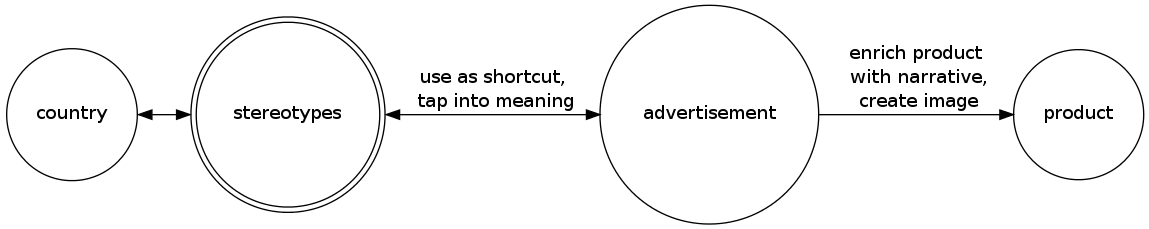
\includegraphics[scale=.4]{concepts.png}
\section{Works Cited}
\include*{biblio}
\end{document}
